\documentclass{bioinfo}
\copyrightyear{2011}
\pubyear{2011}

\usepackage[T1]{fontenc}
\usepackage{amsmath}
\usepackage{amssymb}
\usepackage{natbib}
\usepackage{color} 

%% DEFINE MACROS %%
%% Math macros %%
\newcommand{\prob}{\mathbb{P}}
\newcommand{\odds}{\mathbb{O}}
\newcommand{\likeli}{\mathcal{L}}
\newcommand{\p}{\text{p}}
\newcommand{\expect}{\mathbb{E}}
%% Bio macros %%
\newcommand{\species}[1]{\textit{#1}}
%% Layout macros %%
\newcommand{\remark}[1]{\begin{center}\fcolorbox{black}{yellow}{\parbox{.8\textwidth}{#1}}\end{center}}
\newcommand{\note}[1]{{\color{red}[#1]}}
\newcommand{\REF}{{\color{red}[REF]}}


%%%%%%%%%%%%%%%%%%%%%%%%
%%%%%%% CONTENTS %%%%%%%
%%%%%%%%%%%%%%%%%%%%%%%%

\begin{document}

\firstpage{1}

\title[Bayesian integration of networks without gold standards]{Bayesian integration of networks without gold standards}

\author[J. Weile \textit{et~al.}]{Jochen Weile\,$^{1}$, Katherine James\,$^{1}$, Jennifer Hallinan\,$^{1}$, Simon J Cockell\,$^{2}$, Phillip Lord\,$^{1}$, Anil Wipat\,$^{1,3}$ and Darren Wilkinson\,$^{3,4,}$\footnote{to whom correspondence should be addressed}}

\address{$^{1}$School of Computing Science, $^{2}$Bioinformatics Support Unit, $^{3}$Centre for Integrative Systems Biology of Ageing and Nutrition, $^{4}$School of Mathematics and Statistics, Newcastle University, Newcastle upon Tyne NE1 7RU, United Kingdom}

\history{Received on XXXXX; revised on XXXXX; accepted on XXXXX}

\editor{Associate Editor: XXXXXXX}

\maketitle

\begin{abstract}
\section{Motivation:}
Biological experiments allow insights into networks of processes inside a cell, but are subject to errors. However, thanks to the overlap between the large number of experiments reported in public databases it is possible to assess the chances of individual observations to be correct. In order to do so, existing methods rely on high-quality ``gold standard'' reference networks, but such reference networks are not always available.

\section{Results:}
We present a novel algorithm for computing the probability of experimental observations to be correct that operates without gold standard reference data. We show that our algorithm outperforms existing gold standard based methods. Finally, we apply the new algorithm on a large collection of genetic interaction and protein-protein interaction experiments.

\section{Availability:}
The integrated dataset and a reference implementation of the algorithm as a plug-in for the Ondex data integration framework are available for download at \href{http://bsu.ncl.ac.uk/nogold}{http://bsu.ncl.ac.uk/nogold}.

\section{Contact:} \href{darren.wilkinson@ncl.ac.uk}{darren.wilkinson@ncl.ac.uk}
\end{abstract}

\section{Introduction} 

A significant proportion of knowledge about molecular biological processes is distributed over a large number of online databases \citep{stein_creating_2002}. This knowledge has been obtained through experiments performed in laboratories all over the world. Overlaps often exists across the contents of these databases. The sub-discipline of integrative bioinformatics aims at collating this knowledge and making it accessible to both humans and computers. 

A popular integration paradigm is the construction of functional networks \citep{von_mering_string:_2003,warde-farley_genemania_2010}\note{Also cite Katherine}. Functional networks represent different types of relationships between biological entities in an abstract manner. Associations such as genetic interactions, protein-protein interactions, gene regulation and co-expression are combined into simple abstract statements of functional relatedness, which are termed functional interactions.

An alternative paradigm is semantic data integration \citep{cheung_yeasthub:_2005,smith_obo_2007,koehler_graph-based_2006}. These approaches aim at representing the biological information (and as much of its meaning as possible) in a computationally accessible fashion. Rather than generalizing over all types of associations between entities to infer functional interactions, each type of association is considered separately.

An important question in data integration is how to assess the degree of confidence in each statement, that is, how likely the statement is to be correct. Several popular solutions to this problem exist in the context of functional networks \citep{lee_probabilistic_2004,troyanskaya_bayesian_2003}.
These methods assess the quality of each input dataset against one or more additional datasets of higher quality, usually manually-curated collections. Based on the confidence measures gained from this comparison it is then possible to calculate a confidence measure for each functional interaction. The high-quality datasets used in these comparisons are often referred to as `gold standards'. 

Inferring confidence assessments for semantically integrated datasets is challenging, because each single type of association must be scored separately. However, gold standards only exist for some types of associations. Therefore, it is desirable to find a method that can infer confidence measures on biological networks in the absence of a gold standard, that is, based only on the existing experimental data. So far, only partial solutions to this problem exist. These solutions infer confidence measures for a specific type of association only, for example, protein-protein interactions \citep{bader_gaining_2004}.\note{Find more}

%Whether or not this description is justified is a matter of dispute \REF. 

%It would be desirable to investigate these ideas at a more detailed level, that is, moving on from the question: ``How likely are two given proteins to be functionally related?'', to more specific questions such as: ``How likely is it that two given proteins physically interact?''. However, at this level it becomes infeasible to rely on gold standards, \note{since the level of completeness and quality required has not yet been achieved.} simply because none exist \REF. Therefore, it is necessary to develop a method that can infer confidence measures for semantic statements about molecular biological entities, based only on the existing data.

To provide a more generic solution to this problem, we present a fully Bayesian method which calculates, for each statement in a semantically-integrated dataset, the probability that it is true. We have evaluated the method's effectiveness in comparison to related methods. The validity of any results of the method's application to real data is difficult to verify without knowing the absolute biological truth. Therefore, we have developed a tool that tests integration methods on simulated data with the same characteristics as real biological networks.

\begin{methods}
\section{Methods}

\subsection{Probabilistic integration}

The complete system of processes of a certain type within the cell (e.g. protein-protein interactions) can be modelled as a network $G=(V,E)$, where entities, such as proteins, are nodes (vertices) $V=\{v_1,\ldots,v_N\}$ and their associations are edges $E = \{e_1, \ldots,e_M\} \subseteq \binom{V}{2}$. If one considers each pair of entities to potentially have an edge, it is possible to model the process of prediction of such an edge by an experiment as follows. Let $X = \{X_1, \ldots, X_n \}$ be a collection of $n$ networks which have been experimentally derived from $G$. Considering a single potential edge $e$, each experiment $X_i$ makes a statement about $e$'s existence. Let $D^e_i$ be a random variable that assumes realisation 1 when the $i$th experiment $X_i$ predicts that the edge exists and 0 when it predicts that the edge does not exist. Let $d^e_i$ be the measured realisation from $X_i$, then $(D^e_i=d^e_i)$ is the event that the measured realisation in experiment $i$ is taking place. Furthermore, let $D^e_{(n)}$ be the vector of all $n$ experimental measurement events $(D^e_i=d^e_i)$ for the edge. Finally, let $L^e$ be the event that the edge really does exist in $G$. We are interested in $\prob(L^e|D^e_{(n)})$, that is, the probability that the edge really exists given all our experimental measurements.

An important concept necessary to determine this probability is the Bayes factor \citep{kass_bayes_1995}. For each of the $n$ experiments a Bayes factor $\Lambda_i$ can be determined, which is defined as follows:

\begin{equation} 
	 \Lambda_i := \frac{\prob(D^e_i=d^e_i|L^e)}{\prob(D^e_i=d^e_i|\neg L^e)} 
\end{equation}

If experiment $i$ predicts that the edge exists, then $\Lambda_i$ is the probability of a true positive in $i$ divided by the probability of a false positive in $i$. Otherwise, if $i$ predicts that the edge does not exist, then $\Lambda_i$ is the probability of a false negative in $i$ divided by the probability of a true negative in $i$.

Then, under the assumption that all measurements are independent from each other, the Bayes theorem can be used to show:

\begin{equation} 
	\odds(L^e|D^e_{(n)}) = \Lambda_n \cdot \odds(L^e|D^e_{(n-1)})
\end{equation}

A full proof of the above equation is provided in the supplementary material. This recursive equation can be expressed iteratively as follows:

\begin{equation} 
	\odds(L^e|D^e_{(n)}) = \prod_{i=1}^n \Lambda_i \cdot \odds(L^e)
\end{equation}

That is, the odds of the edge to exist given all the experimental measurements is the product of the Bayes factors for these measurements with the prior odds of edge existence. These odds can be converted into the equivalent probability. 

As mentioned above, the calculation assumes that experimental measurements are stochastically independent. This assumption is not valid for real data, and thus introduces a potential source of error into the methodology. Lee and colleagues address this problem by introducing dependency co-efficients for their datasets, a solution which relies heavily on guesswork \citep{lee_probabilistic_2004}. Instead we focus on making our method robust towards this kind of error. 

\note{TODO: Discuss value of prior odds}

In order to calculate the Bayes factors above it is necessary to determine the rates of false positives and false negatives in each dataset. One approach is to compare each dataset to a gold standard and count the number of differences. However, due to previously discussed lack of gold standards, this approach is not feasible here. Therefore, the only available option is to evaluate the datasets against one another in the form of a common consensus. 

A naive approach is to start with random values for the error rates, and to use them to create a candidate integrated network. Updated parameter values and the resulting integrated networks can then be iteratively computed. However, a series of networks produced by this method does not typically converge to any sensible result (data not shown).

To overcome this problem, a fully Bayesian approach was employed to generate samples from the full joint posterior distribution of $\pi(\theta,G|X)$, where $\theta = \{ (\alpha_1,\beta_1), \ldots , (\alpha_n,\beta_n) \}$ is the vector of error rates associated with the members of the vector of experimental networks $X$, and where $\alpha_i$ is the false positive rate of $X_i$ and $\beta_i$ is the false negative rate of $X_i$..
%This algorithm alternately generates samples of the error rates and of a potential true background graph. The method performs a random walk from one sampled state to another. The more accurate a solution that a particular state represents, the more likely it is to be assumed during the random walk. Thus, averaging over the error rate samples of all steps in the algorithm yields a usable parameter configuration.
%\note{Formalise as way of sampling from full joint posterior. Explain Bayesian inference and Gibbs approach}

%The vector of error rates associated with the members of the vector of experimental networks $X$, is denoted as $\theta = \{ (\alpha_1,\beta_1), \ldots , (\alpha_n,\beta_n) \}$, where $\alpha_i$ is the false positive rate of $X_i$ and $\beta_i$ is the false negative rate of $X_i$.

To determine the joint posterior distribution $\pi(\theta,G|X)$,  one may exploit the following equation:

\begin{equation} 
	 \pi(\theta,G|X) = \frac{\pi(\theta,G,X)}{\prob(X)} 
\end{equation}.

Thus, the posterior distribution $\pi(\theta,G|X)$ is proportional to the joint distribution $\pi(\theta,G,X)$. The joint distribution may in turn be determined as follows.

\begin{equation} 
	 \pi(\theta,G,X) = \pi(G)\cdot\pi(\theta)\cdot\prob(X|\theta,G)
\end{equation}

In summary, the following statement can be made. 

\begin{equation} 
	 \pi(\theta,G|X) \propto \pi(G)\cdot\pi(\theta)\cdot\prob(X|\theta,G) 
\end{equation}

As a consequence, three values need to be determined: the prior distribution $\pi(G)$, the prior distribution $\pi(\theta)$ and the likelihood $\prob(X|\theta,G)$.

We define the prior distribution of $\pi(G)$ based on the prior probability of each single edge to exist:
\begin{align}
  \pi(G) &= \prod_{e \in \binom{V}{2}} \pi(G_e)\\
         &= (1-q)^{\left |\binom{V}{2}\setminus E_G \right |} \cdot q^{|E_G|}
\end{align},
where $q$ is the prior probability of an edge to really exist. \note{Not sure we really need this, since we don't use it afterwards anywhere.}

To determine the prior distribution $\pi(\theta)$, we have to consider the nature of the error rates $\alpha_i$ and $\beta_i$ as ``success rates'' for misreading each potential edge. Modelling each observation event over a potential edge as a Bernoulli experiment with such a success rate, the number of false positives and false negatives in an experimental graph $X_i$ would follow a binomial distribution. The success rates for a binomial distribution can be sampled using the Beta distribution. The Beta distribution is dependent on two parameters, $a$ and $b$. For the prior distribution we assume $a = b = 1$.


\begin{align}
  \alpha_i &\sim Be(a_\alpha, b_\alpha) \; \forall i=1,\ldots,n\\
  \beta_i &\sim Be(a_\beta, b_\beta) \; \forall i=1,\ldots,n
\end{align}.


Since sampling from $\pi(\theta,G|X)$ directly would be very difficult, we instead employ a Gibbs sampling approach \citep{gelfand_sampling-based_1990} and alternately sample from $\pi(\theta|G,X)$ and $\pi(G|\theta,X)$.

The algorithm proceeds in cycles. At the beginning of each new cycle, a potential true graph $G$ needs to be sampled based on the error rate vector $\theta$. The sampling is accomplished by using the Bayesian method discussed above to infer posterior existence probabilities for each edge. These probabilities can then be used to sample a potential $G$ by lookup. That is, for each potential edge, a $\mathcal{U}_{[0,1]}$ random number is sampled. If that random number is smaller than the posterior existence probability of that edge, $G$ will contain the edge. Otherwise $G$ will not contain the edge.

The second step in each cycle is the sampling of a new error rate vector $\theta$ based on $G$. 
As explained above, Beta distributions can be used to describe the behaviour of $\theta$.
The parameters $a$ and $b$ can be interpreted as one plus the number of successes and failures, respectively, in a binomial distributed dataset. In order to obtain values for $a$ and $b$, one can compare each $X_i$ to the currently assumed true graph $G$ and use it to count the number of supposed True Positives (tp), False Positives (fp), True Negatives (tn) and False Negatives (fn). Then, the full conditionals for $\alpha$ and $\beta$ can be sampled as follows:
\begin{align}
  \alpha_i &\sim Be(\text{fp}_i+1, \text{tn}_i+1)\\
  \beta_i &\sim Be(\text{fn}_i+1, \text{tp}_i+1)
\end{align}.

To initiate the algorithm as a whole, we need to generate initial error rate vector $\theta_{\text{init}}$. It is sufficient to sample the initial values for each $\alpha_i$ and $\beta_i$ from their prior distribution.
%$Be(1,1)$, which is equivalent to the uniform distribution $\mathcal{U}_{[0,1]}$. 
Pseudocode for the complete algorithm is given in the supplementary material.

%Finally, a score analogous to the likelihood of the current state can be computed as $\pi(\theta,G|X)$.


\subsection{Evaluation method}

In order to evaluate the method described above and to compare it against other probabilistic integration methods, a simulation and testing environment was created. The testing tool creates a random graph according to a specified model. In the simulation, this graph assumes the role of a true biological graph. The tool then derives a set of graphs from the true graph with pre-determined error rates. In the simulation these graphs assume the role of experimental datasets. 

The simulated experimental datasets are subsequently passed to the integration method under investigation. The integrated graph resulting from the integration method is then compared with the original simulated true graph to evaluate the integration method's performance. Such a testing workflow can be programmed to be executed a large number of times in order to measure a method's average behaviour. Furthermore, the testing tool allows for the automatic variation of different input parameters.

The simulated true graph is created as a scale-free graph using a preferential attachment algorithm, since most molecular-biological graphs have been shown to be approximately scale-free \citep{jeong_lethality_2001, eisenberg_preferential_2003}. A description of the algorithm can be found in the supplementary material.
\note{Mention how this does not match the algorithm's definition of the prior distribution of $G$, thus making it more challenging for the algorithm to perform.}%TODO

The next step consists of the simulation of experimental measurements on the true graph. This is the most crucial step of the artificial testing environment as it is responsible for replicating all the different faults and problems of real data. The simplest type of error occurring in experimental measurements is random noise. This type of error is easily simulated by randomly inserting edges that do not exist in the real data and removing edges that do exist in the real data until the desired error rates are reached. The next problem is systematic error, also known as experimental bias. This phenomenon in particular leads to the violation of stochastic independence between datasets. We simulate this by sampling separate false negative probabilities for each interaction and false positive probabilities for each non-interacting node-pair from Beta distributions. We then use these prepared probilities to generate false positives and false negatives in the experiments, thus introducing the same bias/systematic error. Pseudocode for this method is provided in the supplementary material.
Finally, another type of problem that easily escapes one's attention is the lack of negative records. Most experiments do not report which pairs of nodes do not possess an edge. As a consequence, it is hard to differentiate between node pairs that have been observed not to interact and node pairs that have not been subject to testing. 

After the simulated evidential graphs have been given to the integration method in question the resulting integrated network is evaluated against the original graph. There are a number of different quality measures that can be applied. One important aspect is to measure the accuracy of the method in estimating the error rates in the individual experiments. We can define the quadratic loss for the error estimates as follows:
\begin{equation}
  L_\text{ER} = \frac{1}{2n}\sum_{i=1}^n (\alpha_i - \hat{\alpha_i})^2 + (\beta_i - \hat{\beta_i})^2
\end{equation},
where $\hat{\alpha_i}$ and $\hat{\beta_i}$ are the estimates of the false positive and false negative rates for experiment $i$ according to the integration method in question.

Also, to measure the accuracy of the final edge probabilities produced by the method, we can define further loss functions. Since we can expect a vast number of true negatives when working with sparse, scale-free graphs, it would be helpful to see the loss over interacting and non-interacting node pairs separately. These can be interpreted as analogue to the algorithm's false negative rate and false positive rate:

\begin{align} 
	L^{(+)} &= \frac{1}{|E_G|}\sum_{e \in E_G} (1 - \prob(e \in E_G|X))^2\\
	L^{(-)} &= \frac{1}{|\binom{V}{2} \setminus E_G|}\sum_{e \in \binom{V}{2} \setminus E_G} \prob(e \in E_G|X)^2
\end{align}.

We have evaluated the new algorithm in comparison with two gold standard-based methods presented by Lee and colleagues \citep{lee_probabilistic_2004} and James and colleagues \REF. For our evaluation we have examined the following scenario: Each integration method is given the task of processing a number (3,5,7,9,11) of high-throughput (HTP) experiments with average false negative rate $0.15$ and average false discovery rate of $0.15$ (corresponds to false positive rate of 0.0006). In the case of the gold standard-based methods, one of the input experiments serves as the gold standard.

\subsection{Semantic integration}

In addition to the evaluation on artificial data it is important to analyse the method's performance on real biological data. To this end we have used the semantic data integration system Ondex \citep{koehler_graph-based_2006} to gather as much data as possible on the \species{Saccharomyces cerevisiae} protein-protein interaction (PPI) network. A new PSI-MI 2.5 XML \citep{kerrien_broadening_2007} parser was written to import data from the BioGRID \citep{breitkreutz_biogrid_2008}, MINT \citep{chatr-aryamontri_mint:_2007}, IntAct \citep{hermjakob_intact:_2004} and MIPS-MPACT \citep{guldener_mpact:_2006}. The resulting Ondex dataset represented proteins, their interactions, the experiments in which the interactions have been observed and the publications in which the experiments were described. A semantic merger method was developed to clean the dataset of its redundancies. Further details on the semantic integration procedure can be found in the supplementary material.

\end{methods}

\section{Results}

\subsection{Evaluation on simulated data}

Figure \ref{htp} shows the methods' performances over different numbers of input HTP experiments. It is clearly visible that the new fully Bayesian method overall outperforms both gold standard-based methods. For low numbers of input datasets, the loss over existing interactions is significantly lower. Given more than five HTP experiments, all methods show comparably low loss of existing interactions. 

Regarding non-existing interactions the fully Bayesian method constantly performs better than the method presented by James and colleagues. \note{See if we can get rid of Lee's strange behaviour here, by using a different threshold.}

The average loss regarding the $\theta$ estimates shows the fully Bayesian method's superior precision, which increases with the number of input experiments, while both gold standard-based methods stagnate at constant large amout of loss.

\begin{figure}[!tpb]
\centerline{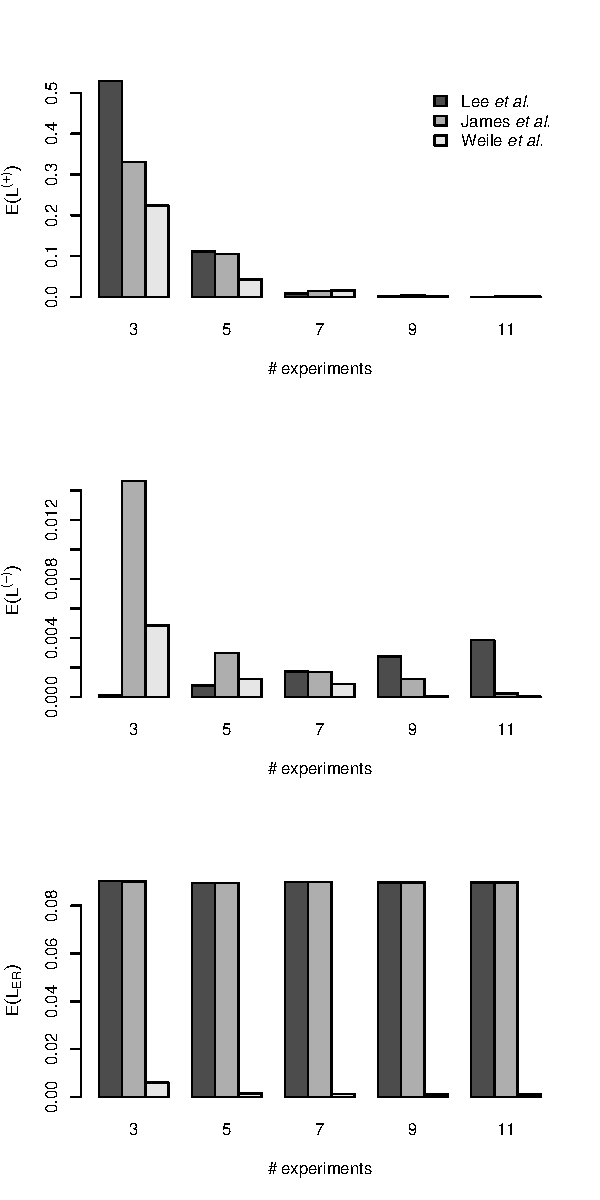
\includegraphics[width=.5\textwidth]{fig1.pdf}}
\caption{Evaluation of the algorithm in comparison with GS-based methods by Lee and colleagues and James and colleagues given different numbers of HTP experiments. Top: Average loss over interacting node pairs ($L^{(+)}$). Centre: Average loss over non-interacting node pairs ($L^{(-)}$). Bottom: Average loss over regarding error rate estimates ($L_\text{ER}$).}
\label{htp}
\end{figure}


\subsection{Application to physical and genetic interactions}

Figure \ref{ppi+gi} shows histograms of the existence probabilities for physical and genetic interactions from the semantically integrated dataset as calculated by the method presented here. A share of 39.03\% of the experimentally reported protein-protein interactions have been assigned probabilites less than 0.1. This percentage is lower than what could be expected according to the projections of Hart and colleagues \citep{hart_how_2006}.


\begin{figure}[!tpb]
\centerline{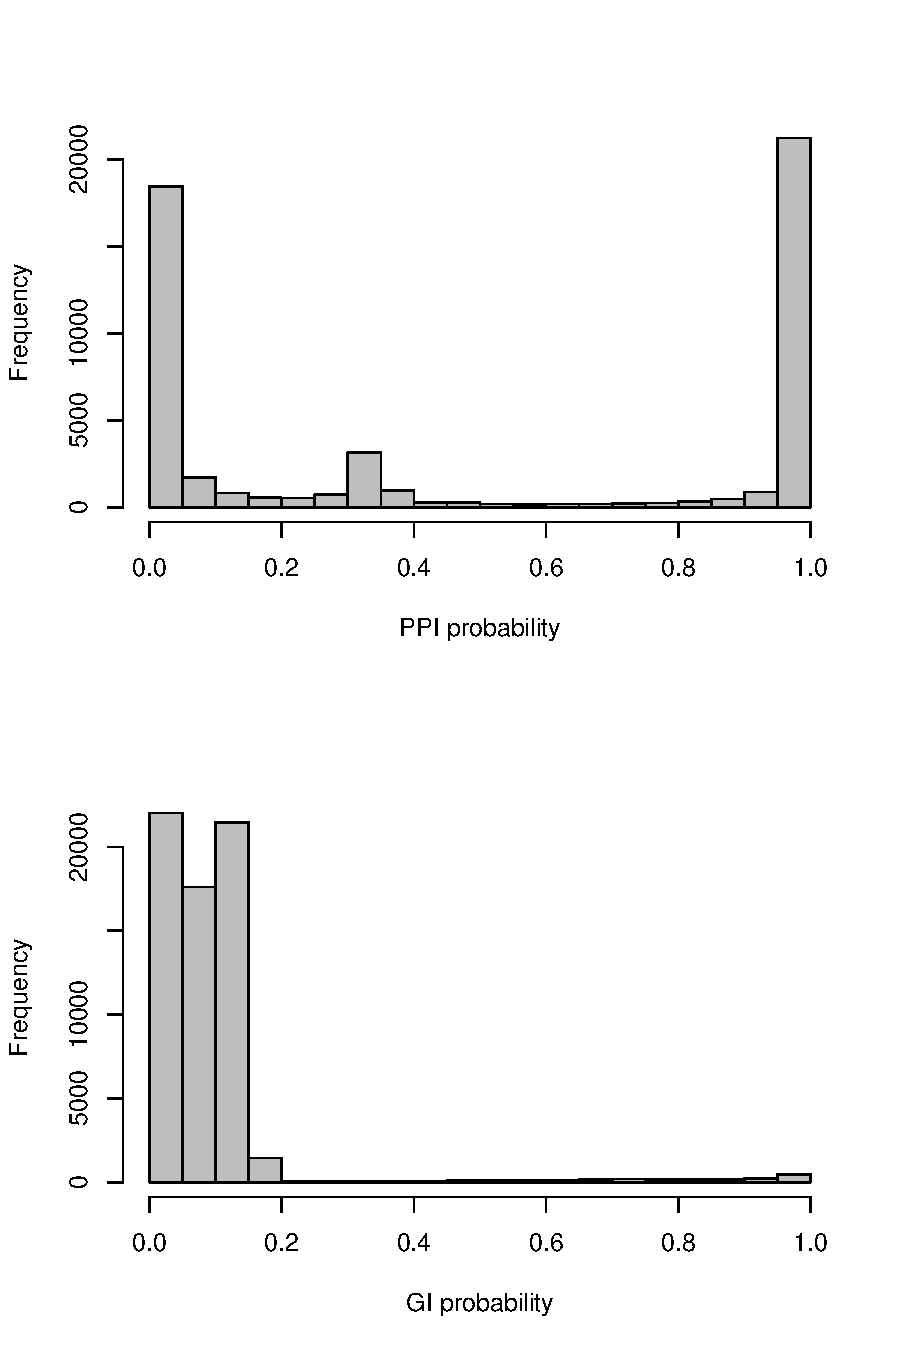
\includegraphics[width=.5\textwidth]{fig2.pdf}}
\caption{Histogram of existence probabilities for the interactions in the integrated dataset. Top: Protein-protein interactions, bottom: genetic interactions.}
\label{ppi+gi}
\end{figure}

%When given a mixed set of HTP and LTP experiments, ...\note{TODO: Implement LTP simulation}

\section{Discussion}
\note{
\begin{itemize}
  \item Excellent performance despite giving competitors head start with unbiased gold standards and accurate fudge factors, which wouldn't be available normally.
  \item Other possible performance metrics (e.g. ROC curves or weighted sums)
  \item Discuss discrepancy between Hart et al and the PPI network
  \item Future work: Evaluate on simulated low-throughput
  \item Future work: Further evaluation of the algorithm using the integrated dataset
  \begin{itemize}
    \item Measure functional annotation accuracy with leave-one-out
  \end{itemize}
\end{itemize}
}

%In addition to the performance metrics used here, others such as the area under ROC curves or weighted sums over the quadratic loss functions above are also possible to apply. However we find that the separate loss functions shown above give a more detailed picture of a method's behaviour.
%\note{Discuss other possible scoring functions, e.g. weighted sums over FPs and FNs}


\section*{Acknowledgements}

\paragraph{Funding\textcolon} The authors are pleased to acknowledge funding from the Biotechnology and Biological Sciences Research Council (BBSRC) Systems Approaches to Biological Research (SABR) initiative (Grant number BB/F006039/1). 

\paragraph{Contributions\textcolon} ...

\paragraph{Conflict of interest\textcolon} None declared.

\bibliographystyle{natbib}

\bibliography{paper}

\note{TODO: Fix capitalization and italics in BibTeX file}

\end{document}
